\section{Evaluation}
\label{sec:eval}

\subsection{Setup}

\paragraph{Real data.} We use 13 series of raw 15\,s scrapes without gaps
from the public Prometheus demo servers~\cite{promdemo}. They include
node\_exporter gauges (load, available memory, free space on the root
filesystem, clock offset), counters and gauges of Prometheus itself, a
Caddy request counter and counters of a demo service. There are two
snapshots, of 7 days (40\,320 samples per series) and 30 days (172\,800
samples). The servers keep only 31 days of data, so we release the
snapshots with the code.

The demo server runs the upstream node-mixin and prometheus-mixin
alerts~\cite{nodemixin}. Nine of them read a single series once constant
denominators are folded into $\theta$. Counters without an upstream rule
get the rules \code{rate(x[5m]) > $\theta$ for 5m} and
\code{rate(x[5m]) < $\theta$ for 10m}. On a healthy host the deployed
thresholds (\code{prod}) never fire. We therefore also run every series
with two recalibrated thresholds, computed from the rule's own aggregate:
the 95th percentile (\code{q95}, an alert that fires often) and the median
(\code{q50}, where the aggregate crosses $\theta$ all the time). Each such
threshold is placed midway between two distinct values, so that discrete
metrics never sit exactly on $\theta$. This gives 26 rule variants per
snapshot, with 1\,864 firings over 7 days and 7\,191 over 30 days.

\paragraph{Synthetic data.} Five seeded generators produce 7 days of
data at 15\,s: CPU utilisation, request latency, memory, a request
counter, and the same counter with 8\,\% missed scrapes, outages of
1--6\,min and traffic that stays close to the threshold. Each dataset has
two rules that fire a few times per day.

\paragraph{Evaluation.} Rules are evaluated every 30\,s, 7\,s after the
scrapes. We compare full alert state trajectories, computed by the
reference evaluator in the repository, which implements Prometheus~3
semantics. Sizes are in bits per value of the value stream, without
timestamps; an uncompressed value takes 64 bits.

\paragraph{Baselines.} Our own configurations all use the same codec and
range coder and differ only in the error budget. \emph{Lossless} is the
codec with a zero budget, which yields Gorilla XOR blocks.
\emph{Uniform-safe} is the largest uniform bound that satisfies
\cref{thm:budget}. \emph{Uniform-tuned} is found by sweeping uniform
bounds over powers of four of the value range: it is the largest bound
such that neither it nor any smaller bound in the sweep changes a decision
\emph{on these data}. A user tuning a bound by hand could do no better,
and the bound guarantees nothing on other data. \emph{SZ3+SG} is
SZ3~\cite{liang2023sz3} wrapped in Compression
Safeguards~\cite{tyree2026safeguards} (1.0.0rc3). It has one stencil
quantity of interest for every window length the rule can read at any
phase, with the comparison itself as the quantity and bound zero. We sweep
13 SZ3 bounds and report the smallest output among those that change no
decision. \emph{Rule-aware} is the analytic budget (\cref{cor:onesided}),
and \emph{$\kappa$} is the optimistic budget with $\kappa = 1024$.

\subsection{Real series}
\label{sec:eval-real}

\begin{table}[t]
\centering
\caption{Mean bits per value over the 13 real series. Zero changed decisions
in every rule-aware cell. ``/120'': Prometheus-sized independent chunks.}
\label{tab:real}
\begin{tabular}{llrrrrrrr}
\toprule
 & rules & lossless & unif.-safe & unif.-tuned & rule-aware & $\kappa$ & rule-aware/120 & $\kappa$/120 \\
\midrule
7\,d  & prod & 27.71 & 0.08 & 0.09 & 0.07 & 0.07 & 0.45 & 0.42 \\
      & q95  & 25.52 & 6.91 & 7.29 & 1.13 & 1.00 & 1.77 & 1.59 \\
      & q50  & 25.52 & 7.69 & 6.01 & 1.49 & 1.38 & 2.16 & 2.00 \\
\midrule
30\,d & prod & 27.77 & 0.08 & 0.08 & 0.06 & 0.06 & 0.44 & 0.41 \\
      & q95  & 25.59 & 7.99 & 5.72 & 0.96 & 0.86 & 1.58 & 1.43 \\
      & q50  & 25.59 & 7.47 & 5.91 & 1.15 & 1.08 & 1.80 & 1.68 \\
\bottomrule
\end{tabular}
\end{table}

\Cref{tab:real} summarises the real data. With the deployed thresholds
nothing fires, and every codec, including the uniform ones, needs less
than 0.1 bits per value, because a threshold that the data never approach
constrains nothing. This is the usual situation in production, but it
does not distinguish the methods. With the recalibrated thresholds, the
rule-aware codec is smaller than the tuned uniform bound by a factor of
6.5 (q95) and 4.0 (q50) on 7 days, and 6.0 and 5.1 on 30 days. Unlike the
tuned bound, it also guarantees the decisions. Per series, its size ranges
from 0.01 bits per value for free filesystem space, which rarely changes,
to 3--4.5 for dense counters under \code{rate} with the median threshold.
In Prometheus-sized chunks of 120 samples, the size grows by 0.6--0.7 bits
per value, mostly because of the fixed overhead per chunk and because the
models start each chunk untrained.

\subsection{Comparison with Compression Safeguards}
\label{sec:eval-sg}

\begin{figure}[t]
\centering
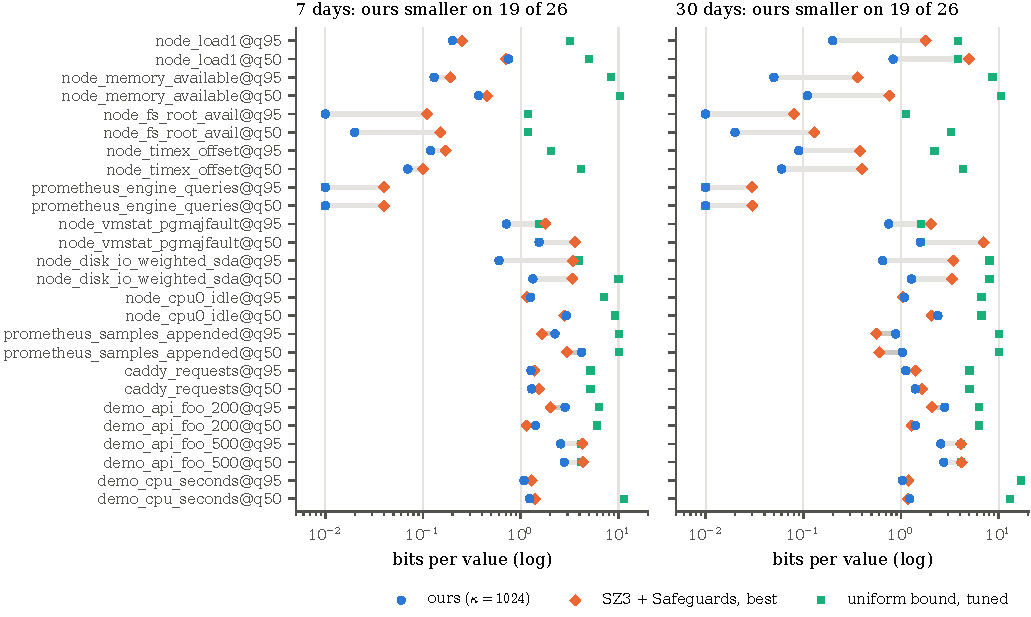
\includegraphics[width=\linewidth]{sg}
\caption{Bits per value on the real series: our optimistic codec
($\kappa = 1024$), the smallest SZ3+SG output with no changed decision over
its bound sweep, and our codec with the largest uniform bound that keeps
every decision on these data (tuned, no guarantee). A grey bar joins ours
to SZ3+SG.}
\label{fig:sg}
\end{figure}

The optimistic codec is smaller than SZ3+SG on 19 of 26 variants in both
snapshots (\cref{fig:sg}). The geometric mean of the size ratio
$\kappa$/SG is 0.60 on 7 days and 0.42 on 30 days. SG stays smaller on
dense counters under \code{rate}
(\code{prometheus\_samples\_appended}, \code{node\_cpu0\_idle} and
\code{demo\_api\_foo\_200}). On these series our quantizer uses one step
for a whole 128-sample block, while SG corrects individual samples.

SG's translation of \code{rate} cannot express Prometheus' extrapolation.
It changed decisions at some sweep points on 4 of the 8 real counters
across the two snapshots, and at 11 of 13 sweep points on the synthetic
counter with missed scrapes. On that counter, the smallest SG output that
keeps every decision takes 8.45 bits per value, 2.9 times more than our
analytic codec (2.91) and 3.1 times more than our optimistic codec (2.74).
A user cannot tell in advance which SG bound is safe. SG needs up to 60\,s per sweep
point on a 30-day counter, while our whole verified codec runs at
11--16\,MB/s (\cref{sec:throughput}).

\subsection{Synthetic series}

\begin{table}[t]
\centering
\caption{Synthetic series, 7 days, bits per value (one stream per series).
SZ3+SG: smallest output with zero changed decisions over its sweep.}
\label{tab:synth}
\begin{tabular}{lrrrrrr}
\toprule
dataset & lossless & unif.-safe & unif.-tuned & SZ3+SG & rule-aware & $\kappa$ \\
\midrule
cpu            & 53.96 & 11.57 & 2.55 & 0.16 & 0.07 & 0.05 \\
latency        & 55.24 &  7.22 & 2.81 & 0.20 & 0.08 & 0.07 \\
memory         & 49.91 & 12.96 & 6.92 & 0.57 & 0.21 & 0.14 \\
requests       & 19.68 &  2.02 & 0.78 & 0.69 & 0.35 & 0.35 \\
requests-gappy & 21.76 & 11.46 & 9.46 & 8.45 & 2.91 & 2.74 \\
\bottomrule
\end{tabular}
\end{table}

On the synthetic gauges (\cref{tab:synth}) the rule-aware codec is
33--36 times smaller than the tuned uniform bound, and on the counters
2.2 and 3.2 times smaller. The analytic codec is smaller than SZ3+SG on
all five datasets. With the box budget of \cref{thm:budget} it was larger
than SZ3+SG on the three gauges, and this result led us to
\cref{cor:onesided}. The size grows with the share of samples near a
threshold: on \code{cpu}, it goes from 0.01 to 0.66 bits per value as that
share goes from 0.1\,\% to 10\,\% (\cref{fig:h2}).

\begin{figure}[t]
\centering
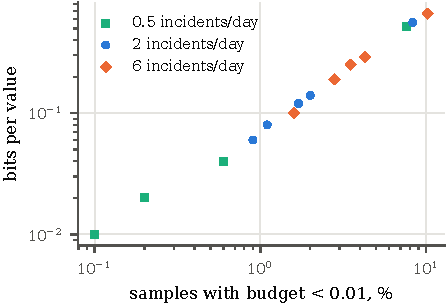
\includegraphics[width=0.5\linewidth]{h2}
\caption{Size of the rule-aware codec on synthetic \code{cpu} (7 days,
one rule) against the share of samples whose budget is below 0.01, for
$\theta \in \{0.55, \dots, 0.95\}$ and three incident rates.}
\label{fig:h2}
\end{figure}

\paragraph{Fidelity.} Without a cap, the reconstruction is useful only
for the rules, since a sample that is free in one direction drifts until
a bound stops it. With a pointwise cap $\eps_{\max}$, the rule-aware
codec is within 2\,\% of the size of a uniform bound $\eps_{\max}$ and
keeps every decision. A uniform bound of $10^{-3}$ of the range changes
17, 929 and 10\,655 alert states on \code{memory}, \code{requests} and
\code{requests-gappy}. Even the tuned uniform bound changes decisions on
two datasets when it is applied to 120-sample chunks instead of the
whole-series encoding it was tuned on. A bound tuned on one encoding of
the data does not carry over to another encoding of the same data.

\subsection{Ablation}
\label{sec:ablation}

\begin{table}[t]
\centering
\caption{Ablation: geometric mean of the size ratio to the full analytic
codec (row 3) over the synthetic series and the q95/q50 real variants
(7-day snapshot; the 30-day snapshot, in the repository, shows the same
ordering). Every cell keeps every
decision.}
\label{tab:ablation}
\begin{tabular}{lrrr}
\toprule
configuration & synthetic & real q95 & real q50 \\
\midrule
box budget, nearest steps (\cref{thm:budget}) & 2.44 & 2.53 & 2.47 \\
\quad + one-sided budget (\cref{cor:onesided}) & 2.27 & 2.06 & 1.91 \\
\quad + lazy steps (full analytic codec) & 1.00 & 1.00 & 1.00 \\
\quad + optimistic budget, $\kappa = 1024$ & 0.80 & 0.92 & 0.95 \\
full analytic + budget-scale search & 1.00 & 1.00 & 1.00 \\
full analytic $-$ one-sided budget & 1.37 & 1.21 & 1.20 \\
full analytic $-$ lazy steps & 2.27 & 2.06 & 1.91 \\
$\kappa = 1024$ $-$ one-sided budget & 0.93 & 1.05 & 1.08 \\
full analytic, fixed-width codes & 8.01 & 7.37 & 5.92 \\
\bottomrule
\end{tabular}
\end{table}

\Cref{tab:ablation} adds one component at a time. With the same stream
format, the one-sided budget and the lazy step choice reduce the size by
a factor of 2.4--2.5 when used together. Either one alone gains much
less. With round-to-nearest, the grid is chosen from the width of the
admissible interval and rounding uses that width symmetrically, so
one-sided bounds alone gain little and sometimes make the output larger.
On counters, all of the gain comes from lazy steps, which keep the
prediction on samples that are not the end of any window
(\cref{prop:rate}(d)). We had also encoded scaled copies of the budget
($\times\frac12, \frac14, \frac18$), because the coded size is not
monotone in the budget. Once the encoder tries the three next finer grids
per block, this search is redundant: it gives a smaller output on none of
the 31 datasets, so the codec no longer does it. The optimistic budget
saves a further 4--20\,\%, but on real data it does not replace the
one-sided budget. Entropy coding avoids the minimum of one bit per value
of fixed-width codes and makes the output 5.9--8.6 times smaller over
both snapshots.

\subsection{Throughput}
\label{sec:throughput}

We measure throughput on one core, in MB/s of raw float64 input, on
synthetic \code{cpu} and \code{requests} with 40\,320 samples. The $O(n)$
budget computation runs at 42--67\,MB/s. The encoder runs at 22\,MB/s,
since every block tries four grids with four step strategies each, and
the decoder at 2.5--2.9\,GB/s. The whole verified compressor runs at
11--16\,MB/s, or 3--4\,MB/s with the budget-scale search, which no longer
changes the size (\cref{sec:ablation}). A 2-hour Prometheus block holds
480 samples per series at 15\,s, so one core compresses about 2\,900
series-blocks per second.
